\section{Model Checking}\label{sec:modelchecking}

\ac{MC} ist eine Möglichkeit, um Systeme zu testen und zu verifizieren. Dazu werden vom \ac{MCr} alle möglichen Systemzustände in einem \emph{brute-force}-ähnlichem Vorgehen getestet und somit alle möglichen Szenarien getestet. Die Anzahl der Zustände kann sehr schnell $ 10^{120} $ oder mehr betragen \cite{Grumberg1999,Baier2008}.

\begin{figure}
	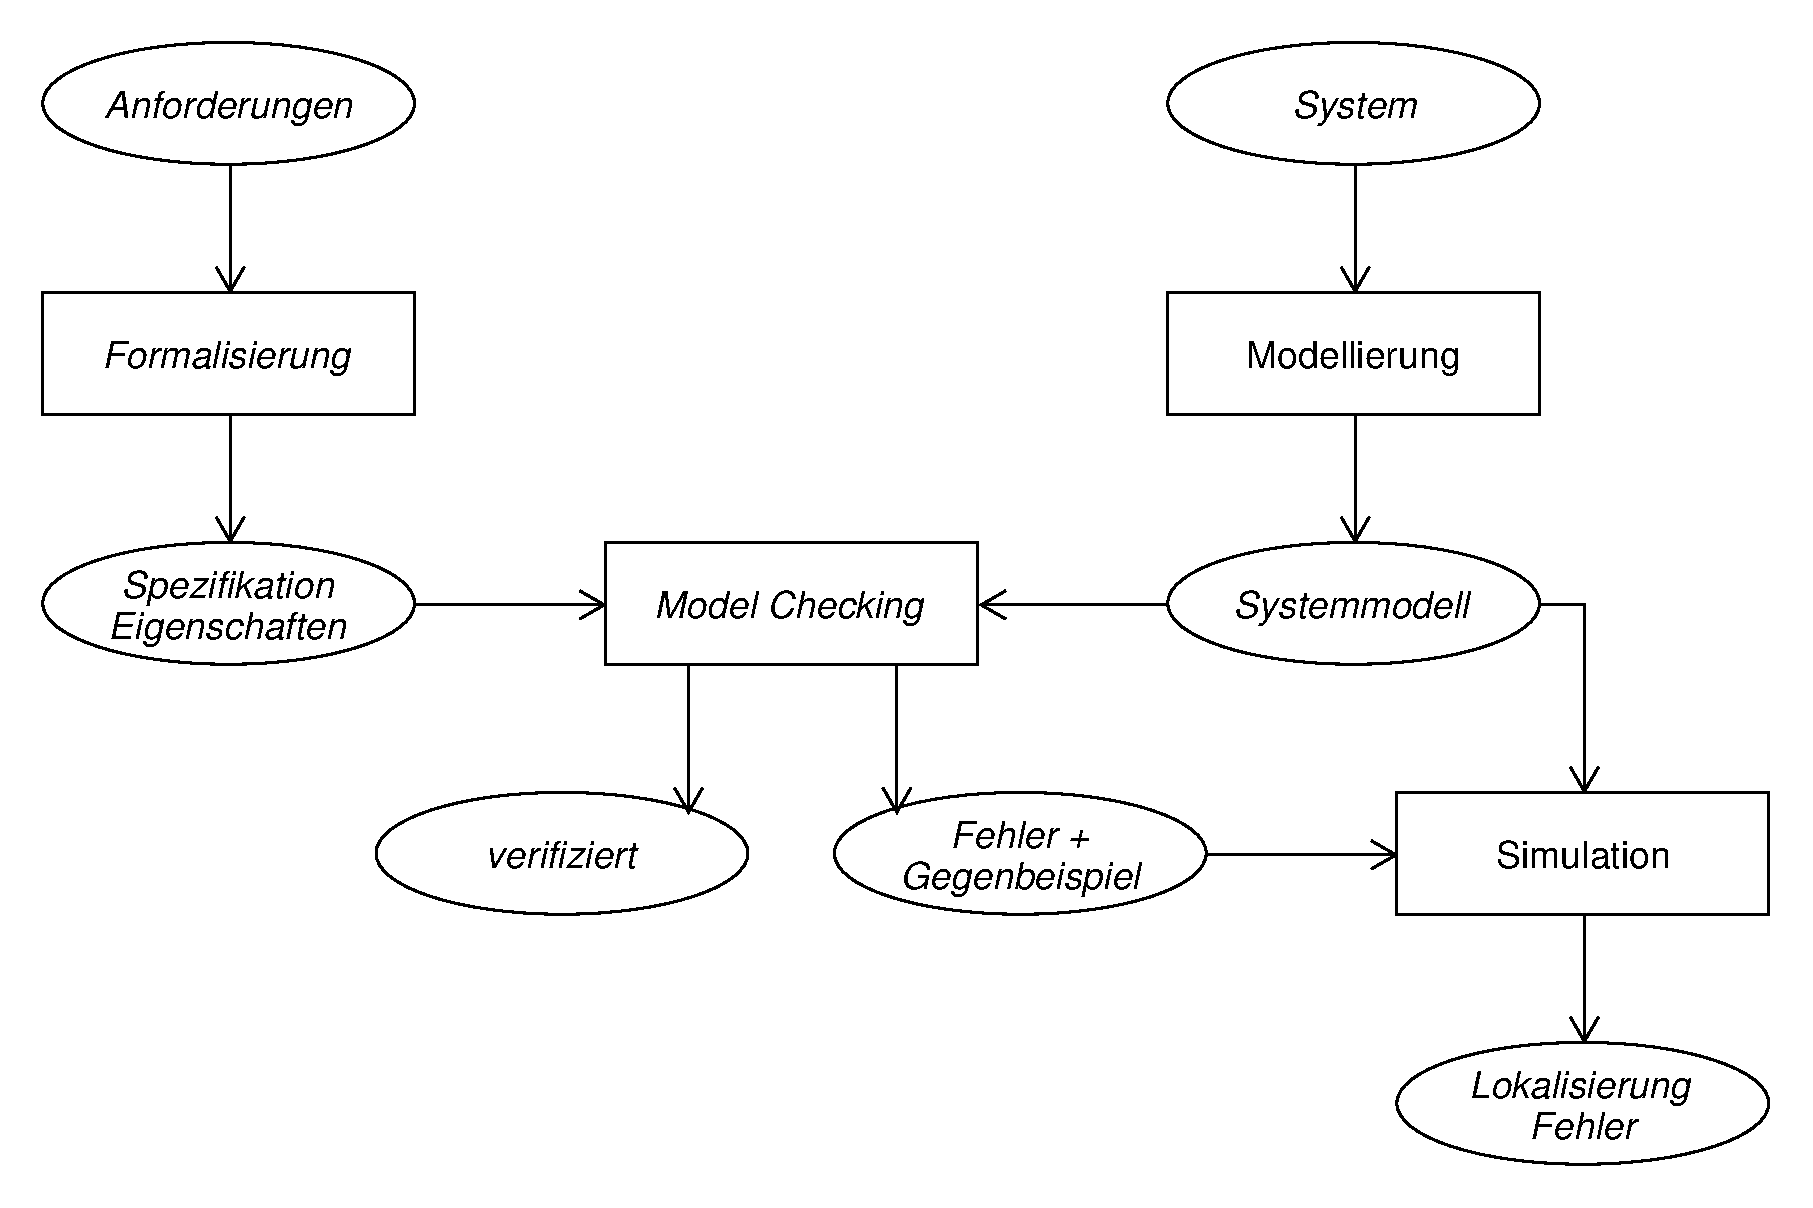
\includegraphics{./images/mcSchema.pdf}
	\caption[Schematischer Aufbau beim MC]{Schematischer Aufbau beim MC, nach \cite{Baier2008}}
	\label{fig:mcSchema}
\end{figure}

Ein \ac{MCr} nutzt, wie der Name schon sagt, ein Modell des Systems, um das System zu testen. Wie bei jeder anderen modellbasierten Technik ist daher die Qualität des \ac{MC} nur so gut wie das darauf zugrunde liegende Modell. Ein Modell kann auch als endlicher Automat angesehen werden, da ein Modell ebenfalls eine endliche Anzahl an möglichen Zuständen und dazugehörige Übergänge besitzt. Für jede Eigenschaft eines Zustandes muss zudem mithilfe einer sog. \emph{temporalen Logik}, also mathematisch bzw. formal, festgelegt werden, was gültige Werte dieser Eigenschaft sind. Die dazu benötigten Informationen werden aus den Anforderungen des Systems ermittelt und dem \ac{MCr} übergeben. So können später verschiedene Eigenschaften des gesamten Systems (\zB die formale Korrektheit, die Ausführbarkeit ohne Deadlocks oder die Einhaltung von Sicherheitsvorgaben) geprüft werden.

Zur Ausführung wird das gesamte Modell zunächst initialisiert und dann automatisch und systematisch vom \ac{MCr} auf Fehler und ungültige Zustände geprüft. In der Regel ist aber auch eine Ausführung als reine Simulation des Systems möglich, ohne explizit nach Fehlern zu suchen.

Wenn alle Zustände und deren Eigenschaften die Anforderungen erfüllen, erfüllt auch das Modell die Spezifikation. Wenn ein Zustand bzw. Eigenschaft die Anforderungen nicht erfüllt, prüft der \ac{MCr} anhand eines Gegenbeispiels den Ausführungspfad zum Fehler. Dadurch kann ermittelt werden, wo die Fehlerursache liegt. Einige der wesentlichen Fehlertypen und Ursachen sind:

\begin{description}
	\item[Modelling Error] Der Fehler liegt im Modell, welches korrigiert werden muss.
	\item[Design Error] Der Fehler liegt in den formellen oder informellen Anforderungen, dadurch muss das Modell und/oder die temporale Logik korrigiert werden.
	\item[Property Error] Der Fehler ist wirklich ein Fehler im System, welcher gefunden werden soll.
\end{description}

Möglich ist aber auch, dass die Ressourcen nicht ausreichen, um alle Zustände zu prüfen. In so einem Fall gibt es mehrere Möglichkeiten, damit umzugehen, \zB können Heuristiken oder Abstraktionen vom Modell genutzt werden \cite{Baier2008,Eberhardinger2016}.

\ac{MC} besitzt durch seine Charakteristik einige Vorteile, \uA \cite{Baier2008}:
\begin{itemize}
	\item \ac{MC} ist universell nutzbar, \zB für Software, Hardware oder eingebettete Systeme
	\item Partielle Verifikation ist möglich ohne das gesamte System testen zu müssen
	\item Vollständig automatisierbar und benötigt kaum Benutzerinteraktion oder hohe Expertise
\end{itemize}

Natürlich gibt es aber auch einige Nachteile, \uA \cite{Baier2008}:
\begin{itemize}
	\item Mit \ac{MC} wird nur ein Systemmodell und nicht das eigentliche System getestet, was weitere Fehler nicht ausschließt
	\item Hauptsächlich für steuerungsbasierte Anwendungen und nicht für datenbasierte Anwendungen geeignet
	\item Anzahl der möglichen Zustände kann zu hoch sein, um alle zu testen
\end{itemize}

Es gibt zahlreiche \ac{MC}-Frameworks, die bereits erwähnten \emph{LTSmin} und \emph{\sS} sind nur zwei davon.